%! Author = natalia
%! Date = 20.02.2020

% Preamble
\documentclass{beamer}

\mode<presentation>
{
\usetheme{Warsaw}
% or Goettingen or Malmoe
\setbeamercovered{transparent}
% or whatever (possibly just delete it)
%\usecolortheme{seahorse}
}

% Packages
\usepackage{amsmath}
\usepackage[english]{babel}
\usepackage[utf8]{inputenc}
\usepackage{graphicx}


\title{Get Good at Git!}
\subtitle{\tiny{(xD)}}
\author{Natalia Maniakowska}
\institute{skygate}
\date{25-02-2020}

\AtBeginSection[]
{
\begin{frame}
    <beamer>{Outline}
    \tableofcontents[currentsection]
\end{frame}
}

\beamerdefaultoverlayspecification{<+->}


% Document
\begin{document}

    \frame{\titlepage}

    \begin{frame}{Outline}
        \tableofcontents
        % You might wish to add the option [pausesections]
    \end{frame}


    %%%%%%%%%%%%%%%%%%%%%%%%%%%%%%%%%%%%%%%%%%%%%%%%
    \section{Introduction}


    \begin{frame}{What is Git? What it isn't?}
        \begin{itemize}
            \item a \textbf{distributed version control system}
            \item created by Linus Torvalds for development of the Linux cernel (2005 -- in, like, a few days!)
            \item free, open source -- GNU General Public License
            \item other DVCS-s: Mercurial, BitKeeper, DCVS\dots (Subversion too, but it's not distributed -- it's centralised)
            \item GitHub $\neq$ Git (!)
        \end{itemize}

    \end{frame}


    \begin{frame}{What is a distributed version control system?}
        \begin{itemize}
            \item \textit{distributed} -- every developer has her/his own copy
            \item \textit{version control} -- keep track of the \textbf{changes}, revert them if needed, etc.
            \item Joel Spolsky\textsuperscript{*} (in 2010): \emph{``possibly the biggest advance in software development technology in the [past] ten years"}
            \href{https://www.joelonsoftware.com/2010/03/17/distributed-version-control-is-here-to-stay-baby}{\beamergotobutton{Article}}

            \footnotesize{(That was actually about Mercurial, but still\dots)}

            \footnotesize{\textsuperscript{*}That guy who invented Trello, Glitch, and co-founded StackOverflow, among others}
        \end{itemize}

    \end{frame}


    \begin{frame}{OK, sounds cool. Let's learn Git.}
        \begin{center}
            So if Git really is so cool and useful, what's the problem with it?

            \href{https://git-man-page-generator.lokaltog.net/}{\beamergotobutton{git manual}}
        \end{center}

    \end{frame}


    %%%%%%%%%%%%%%%%%%%%%%%%%%%%%%%%%%%%%%%%%%%%%%%%%%%%%%%%%%%%%%
    \section{Git Concepts}

    \subsection{Definitions (the absolutely indispensable ones)}


    \begin{frame}
        \frametitle{Git -- definitions}
        \begin{itemize}
            \item repository (repo), .git directory
            \item local vs. remote [repository], origin, upstream
            \item working directory (working tree)
            \item staging area (index)
            \item fetch vs. pull
        \end{itemize}

    \end{frame}


    \begin{frame}
        \begin{figure}
            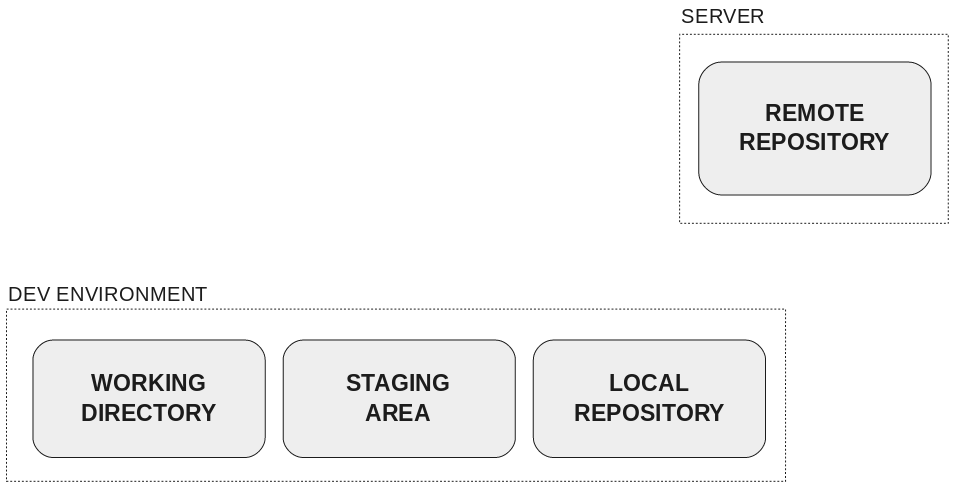
\includegraphics[width=\linewidth]{../figures/general-drawing.png}
            \caption{\footnotesize{A distributed version control system. Source of the picture:
                \href{https://rachelcarmena.github.io/2018/12/12/how-to-teach-git.html}
                {\texttt{https://rachelcarmena.github.io/2018/12/12/how-to-teach-git.html}}}}
        \end{figure}

    \end{frame}


    \begin{frame}
        \frametitle{And more definitions\dots}
        \begin{itemize}
            \item commit, commit hash
            \item branch as a label
            \item \texttt{HEAD} (and \texttt{ORIG\_HEAD}, and \texttt{HEAD\^}, \texttt{HEAD\textasciitilde5}, \dots)
            \item detached HEAD state
        \end{itemize}

    \end{frame}


    \begin{frame}{Rebase}

        \begin{itemize}
            \item \href{https://www.atlassian.com/git/tutorials/merging-vs-rebasing}{Bitbucket tutorial: Merging vs. Rebasing (link)}
            \item \texttt{git rebase --interactive <commit>} -- delete, squash, amend, change the order of, etc. the commits after \texttt{<commit>}
        \end{itemize}

    \end{frame}



    %%%%%%%%%%%%%%%%%%%%%%%%%%%%%%%%%%%%%%%%%%%%%%%%%%%%%%%%%%%%%%

    \subsection{Useful Commands}

    \begin{frame}{Some useful commands}

        \begin{itemize}
            \item \texttt{git config}
                \begin{itemize}
                    \item[$\star$] set editor: \texttt{git config --global core.editor emacs}
                \end{itemize}
            \item \texttt{git status}, \texttt{git log}, \texttt{git diff}, \texttt{git show}
            \item \texttt{git add --patch} (or \texttt{-p}) -- review each changed piece of code and decide whether to add it or not
            \item \texttt{git stash}
            \item \texttt{git reset}
            \item \texttt{git revert}
            \begin{itemize}
                \item[$\star$] see also: \href{https://stackoverflow.com/q/7099833/4744341}{How to revert a merge commit (link)}
            \end{itemize}
            \item \texttt{git cherry-pick}
            \item \texttt{git reflog} -- when something goes terribly wrong
        \end{itemize}

    \end{frame}


    \begin{frame}{A few less crucial, but still useful commands}

        \begin{itemize}
            \item Oh-my-zsh aliases! Do check them out. \href{https://github.com/ohmyzsh/ohmyzsh/wiki/Cheatsheet\#git}{\beamergotobutton{Cheatsheet}}
            \item \texttt{git log --graph --oneline --all}
            \item \texttt{git blame} -- ``annotate" in PyCharm, or a plugin in VS
            \item \texttt{git push --dry-run}
            \item Cleanup (if your repo is getting hefty):
                \begin{itemize}
                    \item[$\star$] \texttt{git gc} -- garbage collection
                    \item[$\star$] \texttt{git remote prune origin} or \texttt{git fetch --all --prune} -- remove
                        references to deleted remote branches (e.g. after they were merged)
                    \item[$\star$] \texttt{git reflog expire --expire=now --all \&\& git gc --prune=now --aggressive}
                        -- erase all Git recovery/backup files (don't use it after \texttt{git reset --hard}!)
                \end{itemize}
        \end{itemize}

    \end{frame}


    %%%%%%%%%%%%%%%%%%%%%%%%%%%%%%%%%%%%%%%%%%%%%%%%%%%%%%%%%%%%%%

    \section{Wrap-up}


    \begin{frame}{Fun facts}

        \begin{itemize}
            \item Git is used in its own development. Git source code is stored on GitHub.
            \item Linux kernel developers don't do pull requests; they send code patches via email.
            Hence \texttt{git format-patch}, \texttt{git send-email}, and other commands.


            \href{https://github.com/torvalds/linux/pull/17\#issuecomment-5654674}{\beamergotobutton{Linus' comment}}
            \item Git also supports octopus merges, which have more than two parents. Probably
                the biggest octopus merge in Linux kernel had 66 (!) parents.

            \href{https://www.destroyallsoftware.com/blog/2017/the-biggest-and-weirdest-commits-in-linux-kernel-git-history}{\beamergotobutton{Article}}
        \end{itemize}

    \end{frame}


    \begin{frame}{Wrap-up}

        Main takeaways:
        \begin{itemize}
            \item \textbf{Never push with \texttt{--force} to public branches!}
            \item It's actually hard to permanently lose some of your work.
            \item Git is cool $\heartsuit$
        \end{itemize}

    \end{frame}


    \begin{frame}
        \frametitle{Questions?}
        \centering
        That's it. Thank you!
    \end{frame}


    \begin{frame}{Resources \& further reading}

        \begin{itemize}
            \item<1-> Rachel M. Carmena, \emph{How to teach Git}
                \href{https://rachelcarmena.github.io/2018/12/12/how-to-teach-git.html}{\texttt{https://rachelcarmena.github.io/2018/12/12/
                how-to-teach-git.html}}
            \item<1-> Nico Riedmann \emph{Learn git concepts, not commands} \href{https://github.com/UnseenWizzard/git_training}{\texttt{https://github.com/UnseenWizzard/git\_training}}
            \item<1-> \href{https://learngitbranching.js.org/}{\texttt{https://learngitbranching.js.org/}} --- an interactive browser ``game'' to learn Git concepts $\heartsuit$
        \end{itemize}

    \end{frame}



\end{document}
